% Options for packages loaded elsewhere
\PassOptionsToPackage{unicode}{hyperref}
\PassOptionsToPackage{hyphens}{url}
%
\documentclass[
]{article}
\usepackage{amsmath,amssymb}
\usepackage{lmodern}
\usepackage{ifxetex,ifluatex}
\ifnum 0\ifxetex 1\fi\ifluatex 1\fi=0 % if pdftex
  \usepackage[T1]{fontenc}
  \usepackage[utf8]{inputenc}
  \usepackage{textcomp} % provide euro and other symbols
\else % if luatex or xetex
  \usepackage{unicode-math}
  \defaultfontfeatures{Scale=MatchLowercase}
  \defaultfontfeatures[\rmfamily]{Ligatures=TeX,Scale=1}
\fi
% Use upquote if available, for straight quotes in verbatim environments
\IfFileExists{upquote.sty}{\usepackage{upquote}}{}
\IfFileExists{microtype.sty}{% use microtype if available
  \usepackage[]{microtype}
  \UseMicrotypeSet[protrusion]{basicmath} % disable protrusion for tt fonts
}{}
\makeatletter
\@ifundefined{KOMAClassName}{% if non-KOMA class
  \IfFileExists{parskip.sty}{%
    \usepackage{parskip}
  }{% else
    \setlength{\parindent}{0pt}
    \setlength{\parskip}{6pt plus 2pt minus 1pt}}
}{% if KOMA class
  \KOMAoptions{parskip=half}}
\makeatother
\usepackage{xcolor}
\IfFileExists{xurl.sty}{\usepackage{xurl}}{} % add URL line breaks if available
\IfFileExists{bookmark.sty}{\usepackage{bookmark}}{\usepackage{hyperref}}
\hypersetup{
  pdftitle={Did COVID-19 cases in Europe lead cases in the USA?},
  pdfauthor={Paul Beaumont   Department of Economics   Florida State University   Tallahassee, FL   {[}beaumont@fsu.edu{]}},
  hidelinks,
  pdfcreator={LaTeX via pandoc}}
\urlstyle{same} % disable monospaced font for URLs
\usepackage[margin=1in]{geometry}
\usepackage{color}
\usepackage{fancyvrb}
\newcommand{\VerbBar}{|}
\newcommand{\VERB}{\Verb[commandchars=\\\{\}]}
\DefineVerbatimEnvironment{Highlighting}{Verbatim}{commandchars=\\\{\}}
% Add ',fontsize=\small' for more characters per line
\newenvironment{Shaded}{}{}
\newcommand{\AlertTok}[1]{\textcolor[rgb]{1.00,0.00,0.00}{#1}}
\newcommand{\AnnotationTok}[1]{\textcolor[rgb]{0.00,0.50,0.00}{#1}}
\newcommand{\AttributeTok}[1]{#1}
\newcommand{\BaseNTok}[1]{#1}
\newcommand{\BuiltInTok}[1]{#1}
\newcommand{\CharTok}[1]{\textcolor[rgb]{0.00,0.50,0.50}{#1}}
\newcommand{\CommentTok}[1]{\textcolor[rgb]{0.00,0.50,0.00}{#1}}
\newcommand{\CommentVarTok}[1]{\textcolor[rgb]{0.00,0.50,0.00}{#1}}
\newcommand{\ConstantTok}[1]{#1}
\newcommand{\ControlFlowTok}[1]{\textcolor[rgb]{0.00,0.00,1.00}{#1}}
\newcommand{\DataTypeTok}[1]{#1}
\newcommand{\DecValTok}[1]{#1}
\newcommand{\DocumentationTok}[1]{\textcolor[rgb]{0.00,0.50,0.00}{#1}}
\newcommand{\ErrorTok}[1]{\textcolor[rgb]{1.00,0.00,0.00}{\textbf{#1}}}
\newcommand{\ExtensionTok}[1]{#1}
\newcommand{\FloatTok}[1]{#1}
\newcommand{\FunctionTok}[1]{#1}
\newcommand{\ImportTok}[1]{#1}
\newcommand{\InformationTok}[1]{\textcolor[rgb]{0.00,0.50,0.00}{#1}}
\newcommand{\KeywordTok}[1]{\textcolor[rgb]{0.00,0.00,1.00}{#1}}
\newcommand{\NormalTok}[1]{#1}
\newcommand{\OperatorTok}[1]{#1}
\newcommand{\OtherTok}[1]{\textcolor[rgb]{1.00,0.25,0.00}{#1}}
\newcommand{\PreprocessorTok}[1]{\textcolor[rgb]{1.00,0.25,0.00}{#1}}
\newcommand{\RegionMarkerTok}[1]{#1}
\newcommand{\SpecialCharTok}[1]{\textcolor[rgb]{0.00,0.50,0.50}{#1}}
\newcommand{\SpecialStringTok}[1]{\textcolor[rgb]{0.00,0.50,0.50}{#1}}
\newcommand{\StringTok}[1]{\textcolor[rgb]{0.00,0.50,0.50}{#1}}
\newcommand{\VariableTok}[1]{#1}
\newcommand{\VerbatimStringTok}[1]{\textcolor[rgb]{0.00,0.50,0.50}{#1}}
\newcommand{\WarningTok}[1]{\textcolor[rgb]{0.00,0.50,0.00}{\textbf{#1}}}
\usepackage{graphicx}
\makeatletter
\def\maxwidth{\ifdim\Gin@nat@width>\linewidth\linewidth\else\Gin@nat@width\fi}
\def\maxheight{\ifdim\Gin@nat@height>\textheight\textheight\else\Gin@nat@height\fi}
\makeatother
% Scale images if necessary, so that they will not overflow the page
% margins by default, and it is still possible to overwrite the defaults
% using explicit options in \includegraphics[width, height, ...]{}
\setkeys{Gin}{width=\maxwidth,height=\maxheight,keepaspectratio}
% Set default figure placement to htbp
\makeatletter
\def\fps@figure{htbp}
\makeatother
\setlength{\emergencystretch}{3em} % prevent overfull lines
\providecommand{\tightlist}{%
  \setlength{\itemsep}{0pt}\setlength{\parskip}{0pt}}
\setcounter{secnumdepth}{5}
\ifluatex
  \usepackage{selnolig}  % disable illegal ligatures
\fi

\title{Did COVID-19 cases in Europe lead cases in the USA?}
\usepackage{etoolbox}
\makeatletter
\providecommand{\subtitle}[1]{% add subtitle to \maketitle
  \apptocmd{\@title}{\par {\large #1 \par}}{}{}
}
\makeatother
\subtitle{An example of TidyR and R Markdown}
\author{Paul Beaumont Department of Economics Florida State University
Tallahassee, FL
{[}\href{mailto:beaumont@fsu.edu}{\nolinkurl{beaumont@fsu.edu}}{]}}
\date{October 07, 2021}

\begin{document}
\maketitle
\begin{abstract}
This is an example of the type of reports that we would like to be able
to produce in this class. Details to follow! For now, we will focus on
the R Studio environment, the yaml, the notion of tidy data, and the
coding conventions that are used here.
\end{abstract}

\begin{Shaded}
\begin{Highlighting}[]
\CommentTok{\# Required libraries}
\FunctionTok{library}\NormalTok{(tidyverse)}
\end{Highlighting}
\end{Shaded}

First, what is the difference between \emph{data science} and \emph{data
analysis}?

Data analysts and data scientists both work with data, but the main
difference lies in what they do with the data. Data analysts examine
large data sets to identify trends, develop charts, and create visual
presentations to help businesses make more strategic decisions. Data
scientists design and construct new processes for data modeling and
production using prototypes, algorithms, predictive models, and custom
analysis.

As an example, we will examine the raw COVID-19 cases data and try to
determine whether cases in Europe led the USA during the initial
outbreak period of February and March of 2020.

The Covid data is from:
\href{https://ourworldindata.org/explorers/coronavirus-data-explorer?time=earliest..2020-04-13\&facet=none\&Metric=Confirmed+cases\&Interval=7-day+rolling+average\&Relative+to+Population=false\&Align+outbreaks=false\&country=USA~Europe~European+Union}{Our
World in Data}.

\begin{Shaded}
\begin{Highlighting}[]
\NormalTok{owid\_covid\_data }\OtherTok{\textless{}{-}} \FunctionTok{read\_csv}\NormalTok{(}\StringTok{"owid{-}covid{-}data.csv"}\NormalTok{)}
\end{Highlighting}
\end{Shaded}

This data comes to us in a ``tidy'' format. By this we mean that the
data are well-organized from a \emph{computing} perspective so that
there are a unique set of identifiers for every data value in the file.
Humans prefer to see ``flat'' files like spreadsheets but this is very
often inefficient from a computing perspective because we have to
continually reformat and reorganize the data for different types of
analyses.

Putting the data into a tidy format can be quite tedious and needs to be
carefully thought out from the beginning. This is the job of a data
scientist. Their tool of choice is usually SQL, which you may have had
some exposure to. We will spend quite a bit of time learning about the
\emph{tidyverse} which is a simplified, but more user friendly, version
of SQL developed within R.

As data analysts, we hope that our data is already tidy, or can easily
be made tidy, so we really want to focus on how to manipulate tidy data
to do useful analyses. For our example, we will select the total cases
and the ``seven day moving average of new cases'' for Europe, European
Union, and the United States from the beginning of the data set (
2020-02-01) through 2020-03-31.

\begin{Shaded}
\begin{Highlighting}[]
\NormalTok{USEU }\OtherTok{\textless{}{-}}\NormalTok{ owid\_covid\_data }\SpecialCharTok{\%\textgreater{}\%}
  \FunctionTok{filter}\NormalTok{(}
\NormalTok{    location }\SpecialCharTok{\%in\%} \FunctionTok{c}\NormalTok{(}\StringTok{"Europe"}\NormalTok{, }\StringTok{"European Union"}\NormalTok{, }\StringTok{"United States"}\NormalTok{) }\SpecialCharTok{\&}
\NormalTok{      date }\SpecialCharTok{\textgreater{}=} \StringTok{"2020{-}02{-}01"} \SpecialCharTok{\&}\NormalTok{ date }\SpecialCharTok{\textless{}=} \StringTok{"2020{-}03{-}31"}
\NormalTok{  ) }\SpecialCharTok{\%\textgreater{}\%}
  \FunctionTok{select}\NormalTok{(location, date, total\_cases, new\_cases\_smoothed)}
\end{Highlighting}
\end{Shaded}

First we plot the total cases data. It ``looks'' like Europe and the EU
lead the USA.

\begin{Shaded}
\begin{Highlighting}[]
\NormalTok{USEU }\SpecialCharTok{\%\textgreater{}\%}
  \FunctionTok{ggplot}\NormalTok{(}\AttributeTok{mapping =} \FunctionTok{aes}\NormalTok{(}
    \AttributeTok{x =}\NormalTok{ date,}
    \AttributeTok{y =}\NormalTok{ total\_cases,}
    \AttributeTok{group =}\NormalTok{ location,}
    \AttributeTok{color =}\NormalTok{ location}
\NormalTok{  )) }\SpecialCharTok{+} \FunctionTok{geom\_line}\NormalTok{() }
\end{Highlighting}
\end{Shaded}

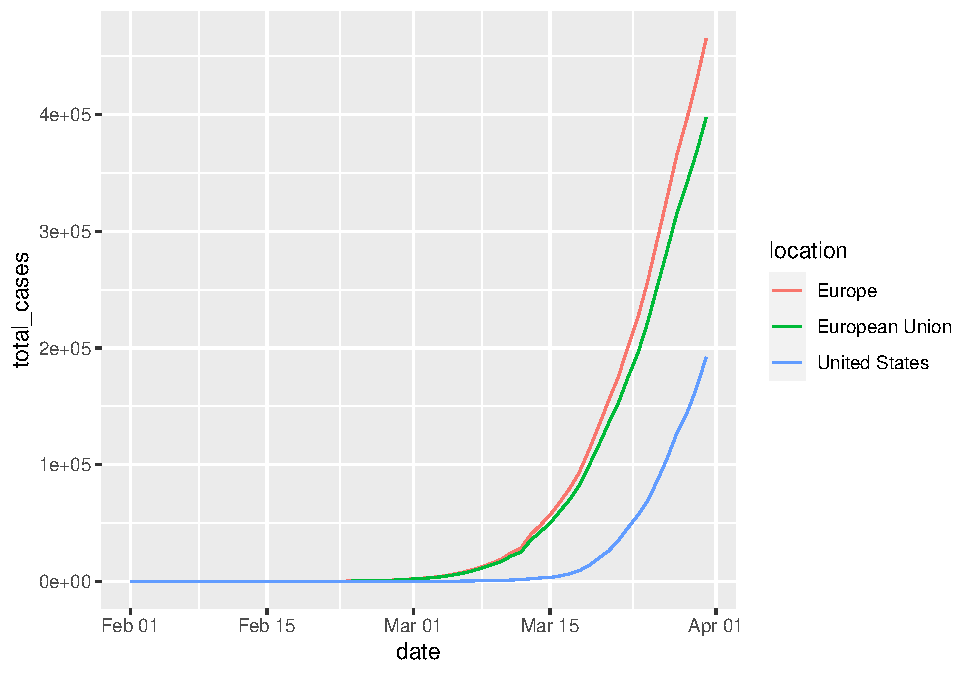
\includegraphics{covid_files/figure-latex/unnamed-chunk-4-1.pdf}

One statistical issue is that the total\_cases data are clearly
\emph{non-stationary}. This is a common problem that we will have a lot
to say about in the class. For now, we will deal with this issue by
examining the percentage change in total\_cases.

\begin{Shaded}
\begin{Highlighting}[]
\NormalTok{USEU\_pct }\OtherTok{\textless{}{-}}\NormalTok{ USEU }\SpecialCharTok{\%\textgreater{}\%}
  \FunctionTok{group\_by}\NormalTok{(location) }\SpecialCharTok{\%\textgreater{}\%} 
  \FunctionTok{mutate}\NormalTok{(}\AttributeTok{pct =} \DecValTok{100}\SpecialCharTok{*}\NormalTok{(}\FunctionTok{log}\NormalTok{(total\_cases}\SpecialCharTok{/}\FunctionTok{lag}\NormalTok{(total\_cases))))}
\end{Highlighting}
\end{Shaded}

\begin{Shaded}
\begin{Highlighting}[]
\NormalTok{USEU\_pct }\SpecialCharTok{\%\textgreater{}\%} 
  \FunctionTok{ggplot}\NormalTok{(}\AttributeTok{mapping =} \FunctionTok{aes}\NormalTok{(}
    \AttributeTok{x =}\NormalTok{ date,}
    \AttributeTok{y =}\NormalTok{ pct,}
    \AttributeTok{group =}\NormalTok{ location,}
    \AttributeTok{color =}\NormalTok{ location}
\NormalTok{  )) }\SpecialCharTok{+} \FunctionTok{geom\_line}\NormalTok{()}
\end{Highlighting}
\end{Shaded}

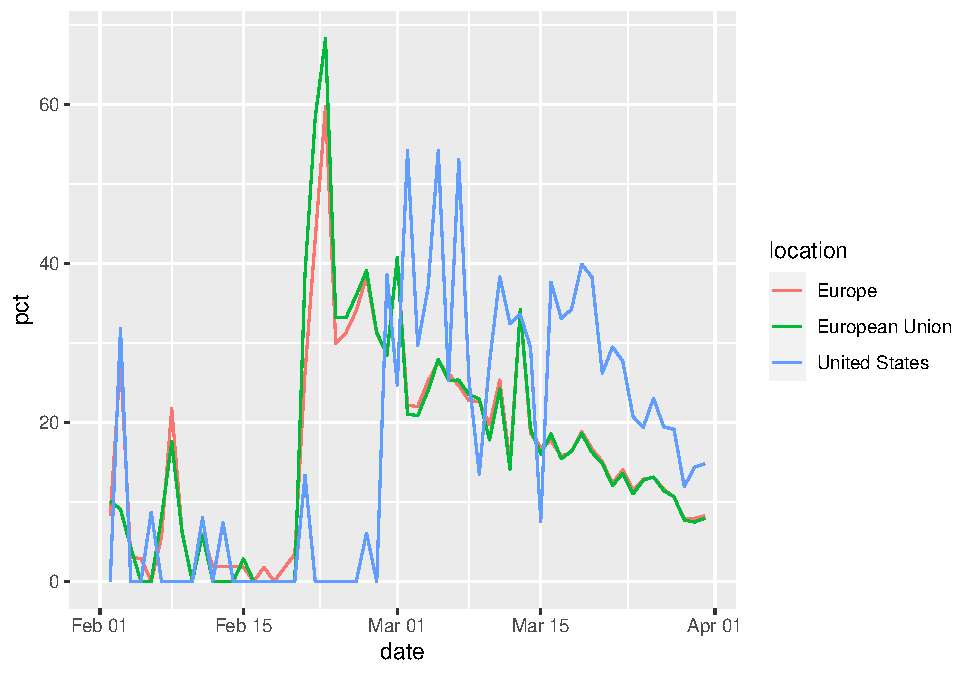
\includegraphics{covid_files/figure-latex/unnamed-chunk-6-1.pdf}

From a statisticians viewpoint, that looks much nicer.

Now we will compute the cross-correlation function for the growth rate
of total cases in the USA and in Europe.

\begin{Shaded}
\begin{Highlighting}[]
\NormalTok{usa }\OtherTok{\textless{}{-}}\NormalTok{ USEU\_pct }\SpecialCharTok{\%\textgreater{}\%} 
  \FunctionTok{filter}\NormalTok{(location }\SpecialCharTok{==} \StringTok{"United States"}\NormalTok{) }\SpecialCharTok{\%\textgreater{}\%} 
\NormalTok{  ungroup }\SpecialCharTok{\%\textgreater{}\%} 
  \FunctionTok{select}\NormalTok{(date, pct) }\SpecialCharTok{\%\textgreater{}\%} 
  \FunctionTok{drop\_na}\NormalTok{()}
\NormalTok{europe }\OtherTok{\textless{}{-}}\NormalTok{ USEU\_pct }\SpecialCharTok{\%\textgreater{}\%} 
  \FunctionTok{filter}\NormalTok{(location }\SpecialCharTok{==} \StringTok{"Europe"}\NormalTok{) }\SpecialCharTok{\%\textgreater{}\%} 
\NormalTok{  ungroup }\SpecialCharTok{\%\textgreater{}\%} 
  \FunctionTok{select}\NormalTok{(date, pct) }\SpecialCharTok{\%\textgreater{}\%} 
  \FunctionTok{drop\_na}\NormalTok{()}
\end{Highlighting}
\end{Shaded}

\begin{Shaded}
\begin{Highlighting}[]
\NormalTok{ccf.out }\OtherTok{\textless{}{-}}
  \FunctionTok{ccf}\NormalTok{(usa}\SpecialCharTok{$}\NormalTok{pct,}
\NormalTok{      europe}\SpecialCharTok{$}\NormalTok{pct,}
      \AttributeTok{lag.max =} \DecValTok{14}\NormalTok{,}
      \AttributeTok{plot =} \ConstantTok{FALSE}\NormalTok{)}
\CommentTok{\# find the h for the maximum cross{-}correlation}
\NormalTok{h\_max }\OtherTok{\textless{}{-}} \FunctionTok{which}\NormalTok{(ccf.out}\SpecialCharTok{$}\NormalTok{acf }\SpecialCharTok{==} \FunctionTok{max}\NormalTok{(ccf.out}\SpecialCharTok{$}\NormalTok{acf))}
\NormalTok{max\_ccf\_lag }\OtherTok{\textless{}{-}}\NormalTok{ ccf.out}\SpecialCharTok{$}\NormalTok{lag[h\_max]}
\NormalTok{max\_ccf\_value }\OtherTok{\textless{}{-}}\NormalTok{ ccf.out}\SpecialCharTok{$}\NormalTok{acf[h\_max]}
\CommentTok{\# plot the ccf}
\FunctionTok{plot}\NormalTok{(ccf.out, }\AttributeTok{ylab =} \StringTok{"cross{-}correlation"}\NormalTok{, }\AttributeTok{main =} \StringTok{"CCF: USA(t) vs. Europe(t{-}h)"}\NormalTok{)}
\end{Highlighting}
\end{Shaded}

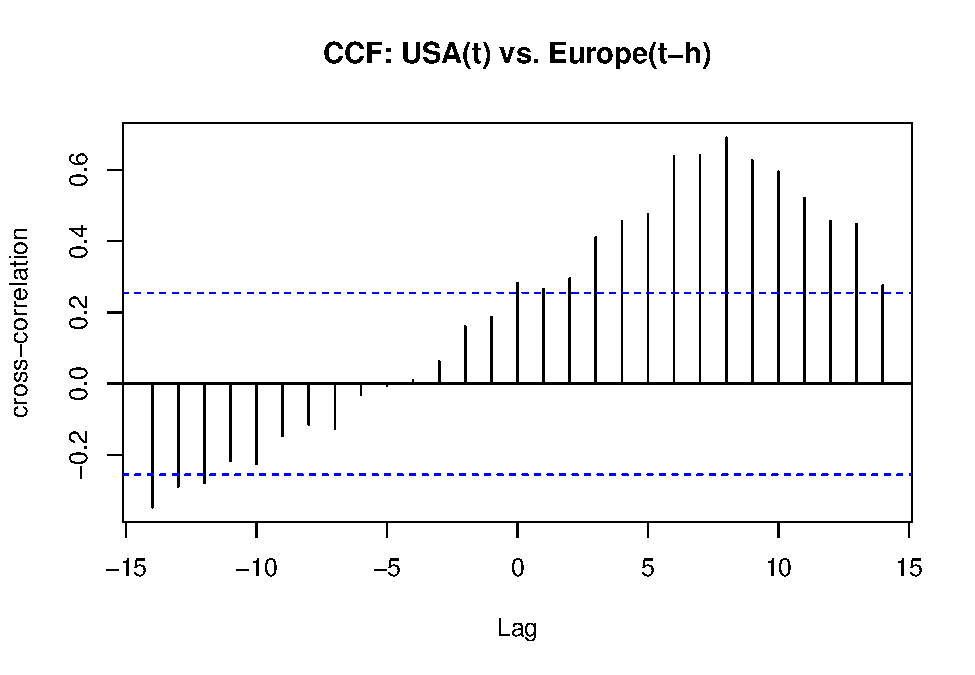
\includegraphics{covid_files/figure-latex/unnamed-chunk-8-1.pdf}

The CCF plot suggests that the growth rate of the number of cases in
Europe leads the USA with a maximum cross-correlation of 0.69 at 8 days.

\end{document}
